\chapter{Implementación}
\section{Introducción}

En este capítulo se describirá la implementación del proyecto, dando énfasis en las tecnologías y dispositivos usados para el posicionamiento.

\section{Implementación general de trabajo}
A continuación, se observa el esquema general del algoritmo a implementar y cómo confluyen ambas partes para llevar a cabo el posicionamiento.

\begin{figure}[h!]
    \centering
    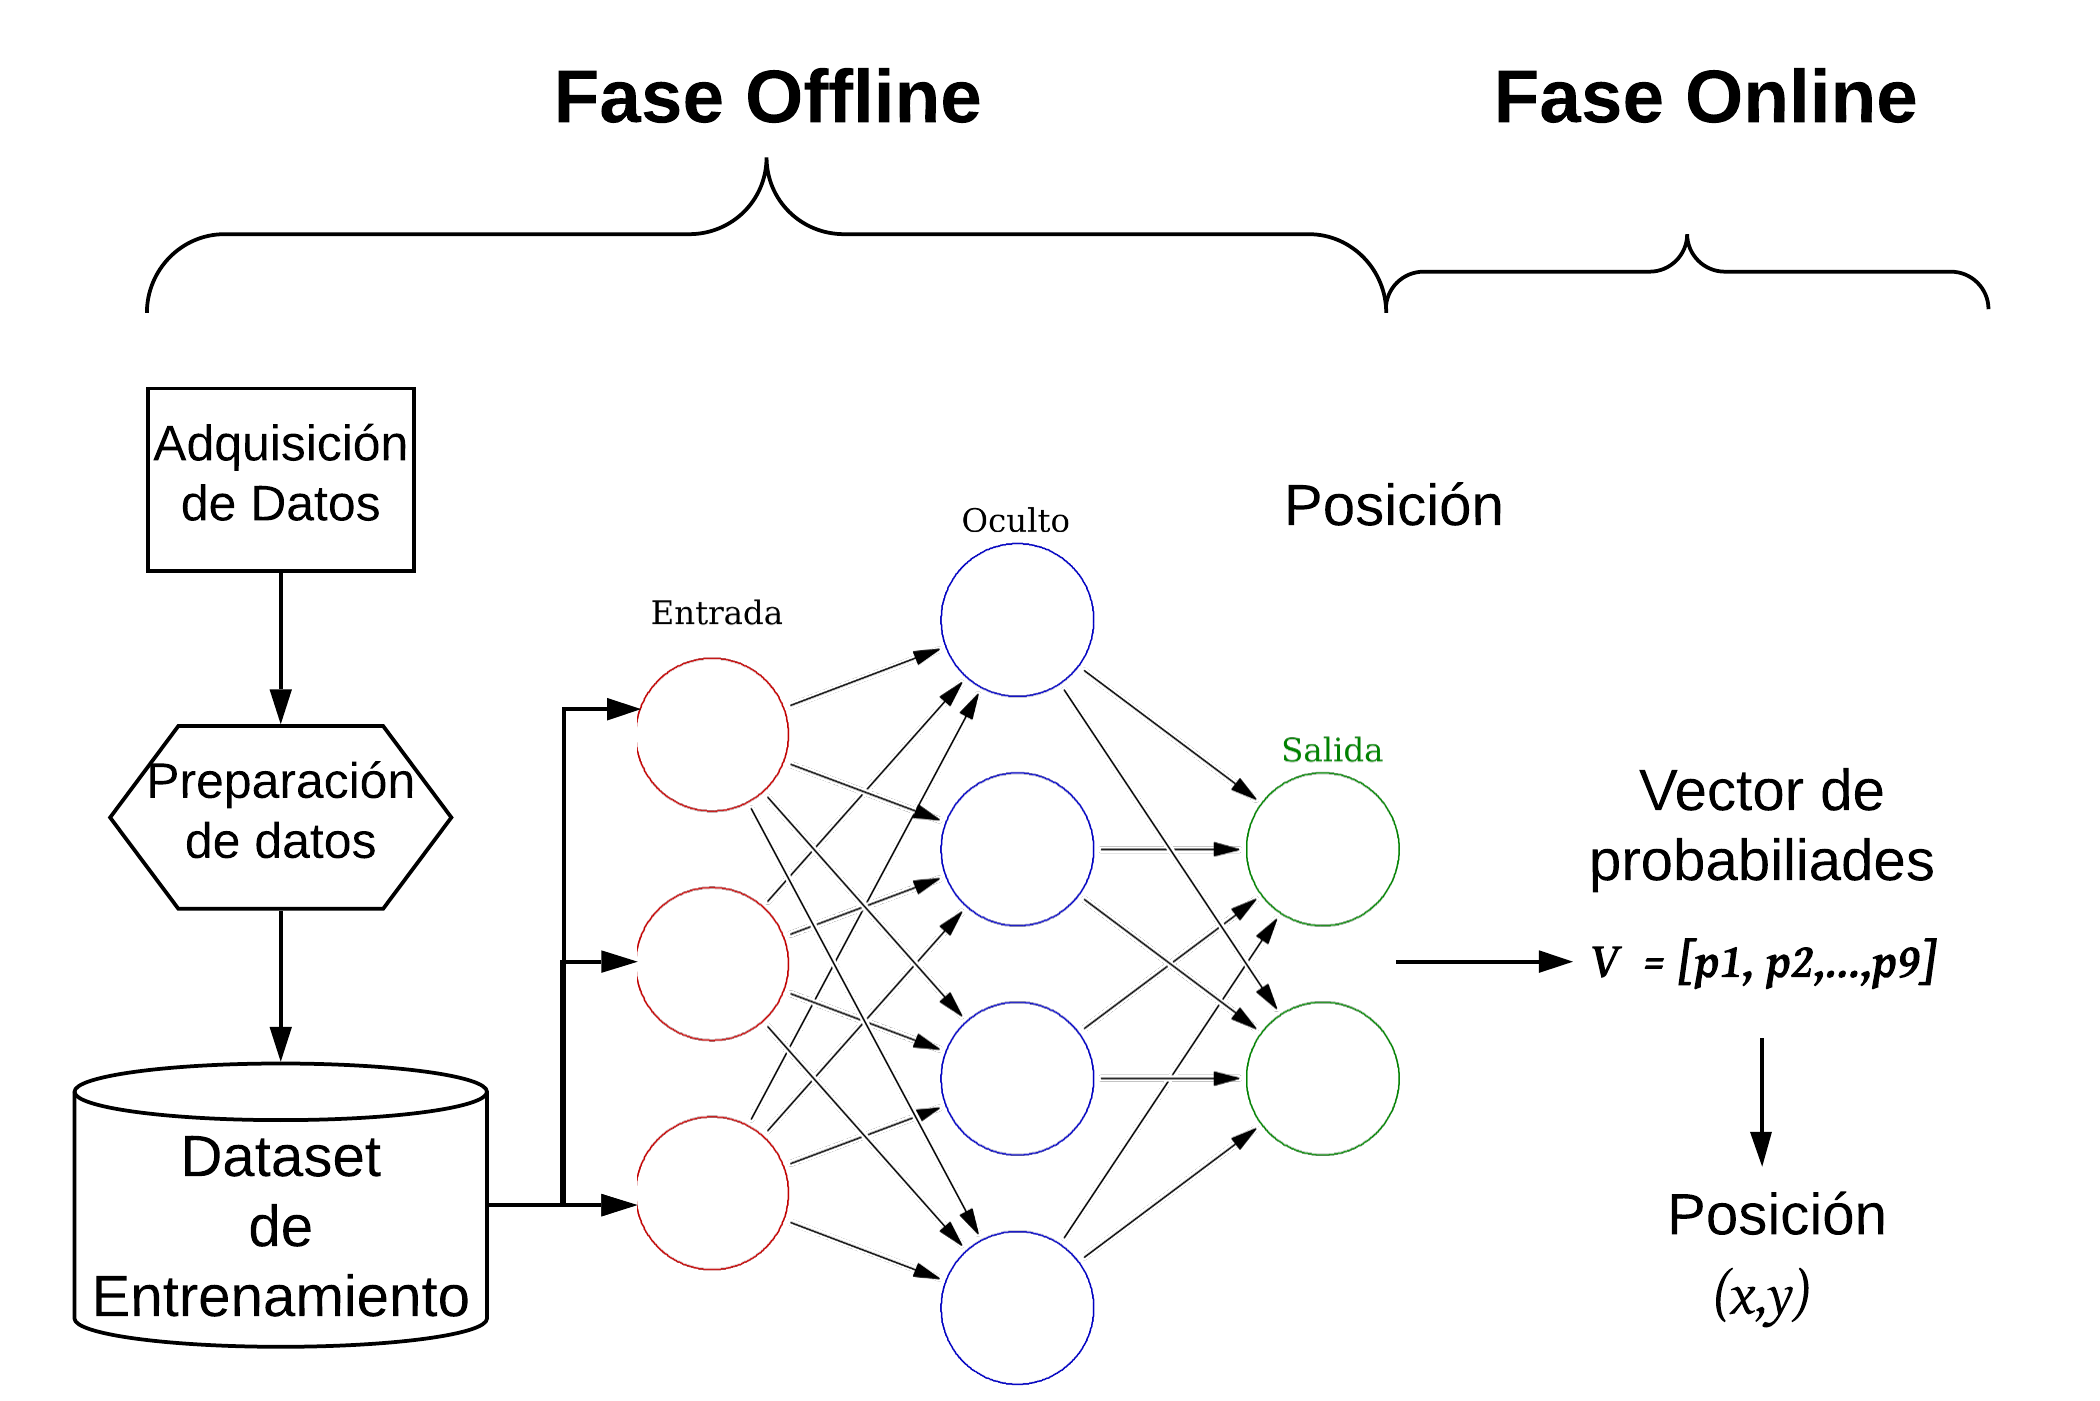
\includegraphics[scale=0.15]{./images/esquema2}
    \caption{Esquema de Implementación General de Trabajo}
    \label{fig:esquema2}
\end{figure}


\subsection{Fase Offline}
\subsubsection{Adquisición de RSSI}
La adquisición de estos datos se hará con la librería de linux llamada \texttt{iwlist}. Una breve descripción de esta, a continuación:

\begin{itemize}
    \item{\textbf{Descripción}: Iwlist es usada para mostrar información adicional de dispositivos inalámbricos de una red. El argumento principal es usado para seleccionar una categoría de información, \texttt{iwlist} muestra información en detalle para toda la información relacionada a esta categoría, incluyendo la información que se muestra en \texttt{iwconfig}.}
    
    \item {\texttt{Scan}: Entrega una lista completa de los Access Points y celdas Ad-Hoc en el rango, y opcionalmente, información adicional sobre ellos. Algunos de estos datos adicionales son \texttt{ESSID, Quality, Frequency, Mode, etc} que permiten entre otras cosas, reconocer la \textbf{dirección MAC} de los dispositivos, el \textbf{RSSI}, y el \textbf{nombre de la red}.
    
    \begin{figure}[h!]
        \centering
        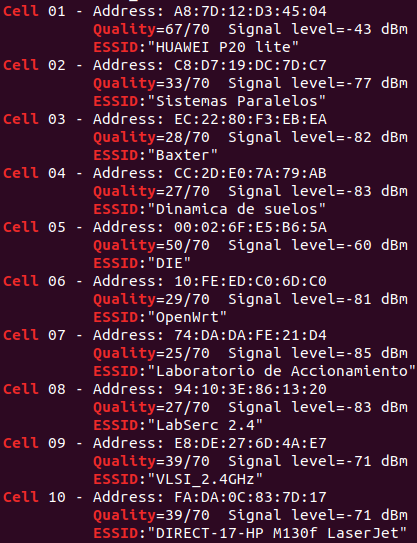
\includegraphics[scale=0.5]{./images/output}
        \caption{Salida de consola con datos de AP}
        \label{fig:output}
    \end{figure}
    
    En esta parte, es necesario recalcar que las características a desplegar dependerán de la tarjeta de red de manera que para efectos del proyecto, se limitarán al adaptador de red inalámbrico conectado a la raspberry pi}
\end{itemize}

Con lo mencionado anteriormente podemos hacer un mapeo del laboratorio tal que para una posición específica sea, por ejemplo $(x,y) = (0,0)$ el punto de origen de las mediciones, puedan obtenerse los niveles de intensidad de señal. De este modo, extendiendo esta metodología a las demás posiciones es que se caracterizará el espacio en función del parámetro RSSI en \ref{fig:esquema}.

Las mediciones se harán en espacio accesible y de trafico relativamente bajo como es el laboratorio de redes de datos. Este para efectos prácticos fue dividido en dos partes como se presenta en la siguiente imagen:

\begin{figure}[h!]
    \centering
    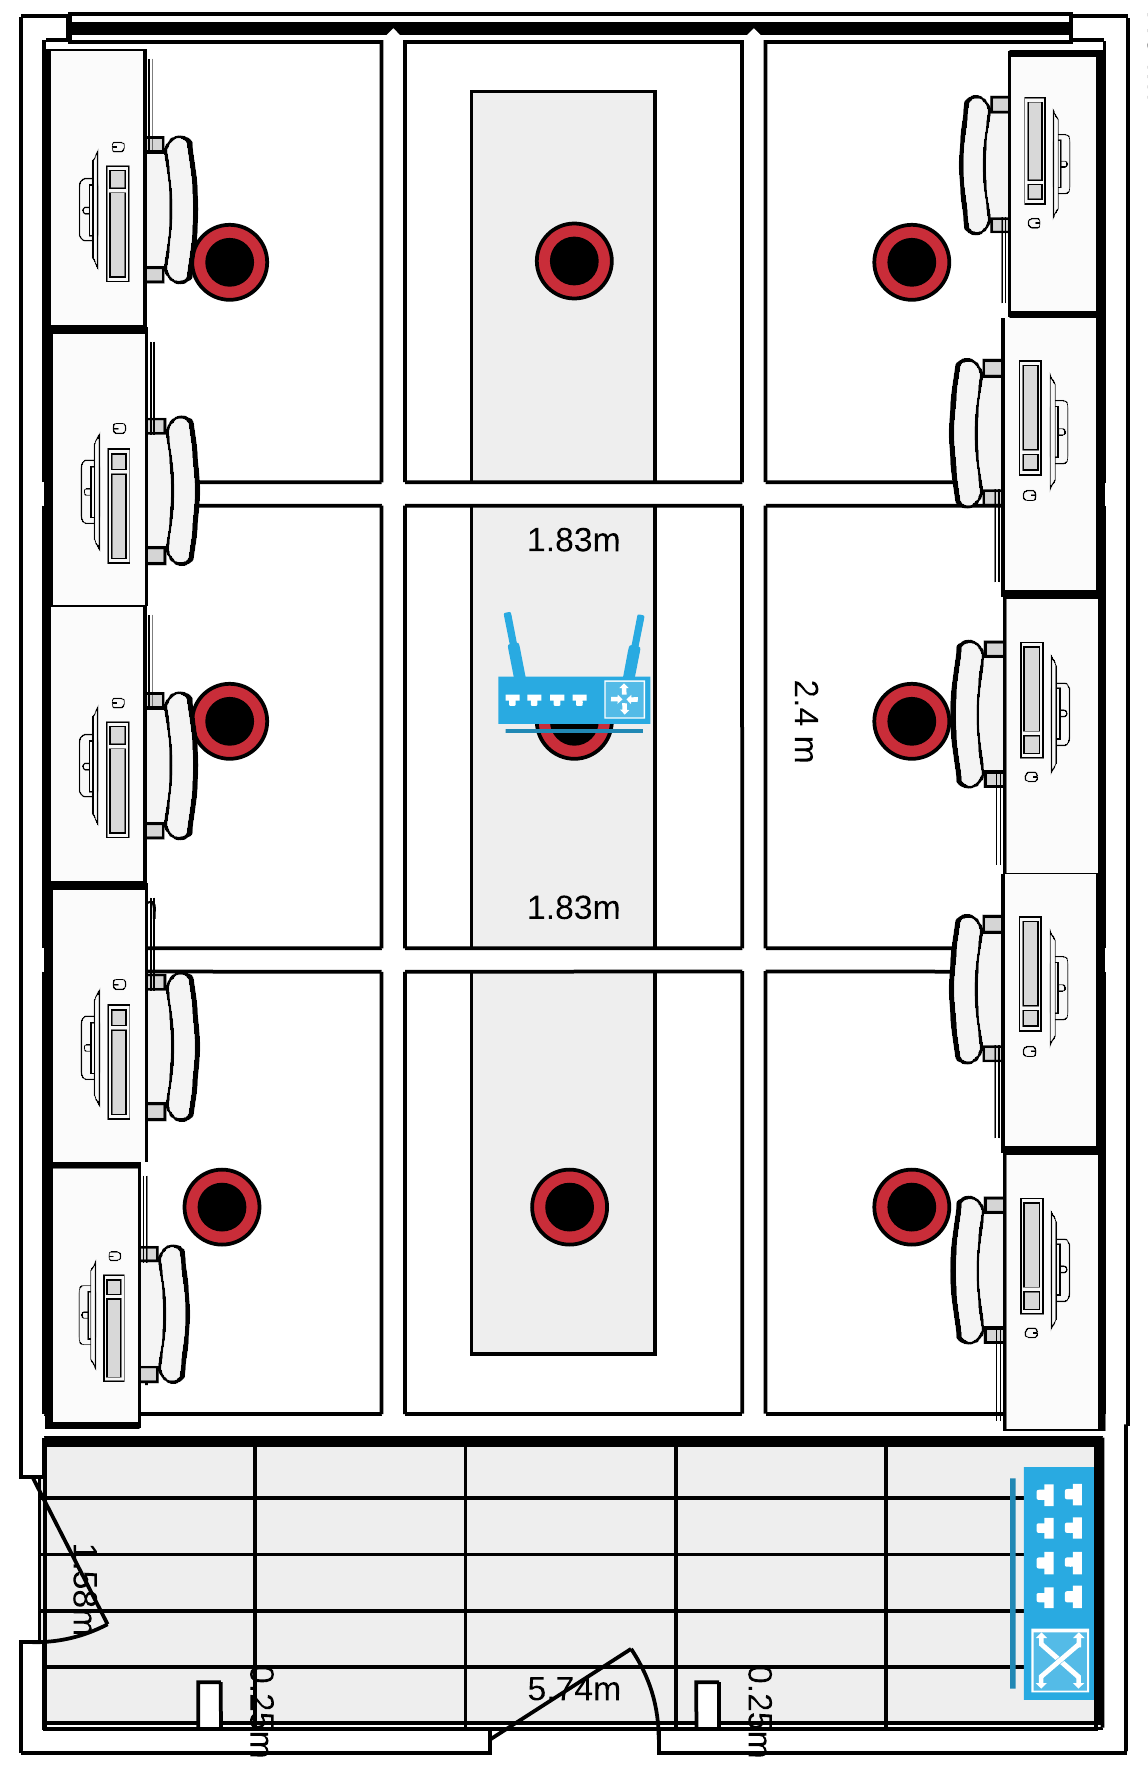
\includegraphics[angle=90,origin=c,scale=0.2]{./images/maplab}
    \caption{Mapa Lab. de Redes de datos}
    \label{fig:mapalab}
\end{figure}

\begin{itemize}
    \item {\textbf{Escritorios y computadores}: corresponden a la parte que no está ennegrecida y que fue dividida en 9 sectores de 2.4 x 1.83 m en los cuales se dispusieron los equipos -representados a través de los puntos rojos con negro, a una altura de 0.8 m para así medir. Estos fueron ubicados equidistantes uno de otro.}
    \item{\textbf{Franja no utilizable}: este sector corresponde a un espacio que dada su relación asimétrica de profundidad y densidad de materiales no fue considerado en el estudio.}
\end{itemize}

\subsubsection{Set de entrenamiento}
En esta parte, los datos son filtrados, separados y agrupados en un archivo \texttt{.csv} para la posterior lectura y procesamiento de la Red Neuronal.

El formato de los datos de entrada proveídos a la red es el siguiente.
\begin{figure}[h!]
    \centering
    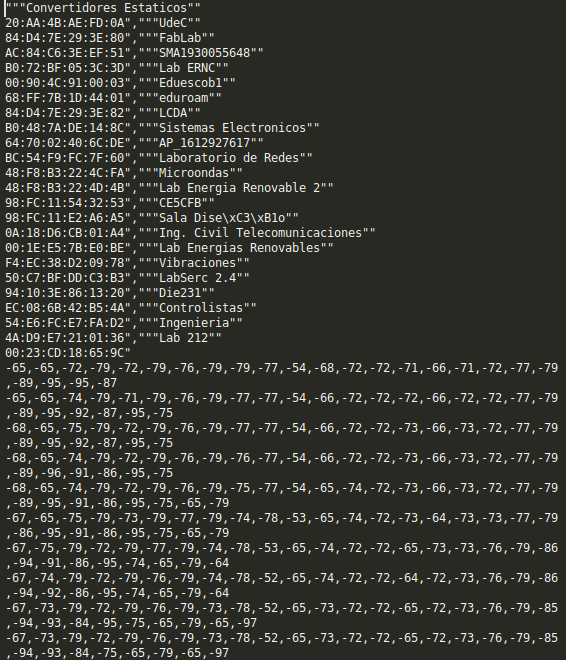
\includegraphics[scale=0.5]{./images/plaincsv}
    \caption{Formato tipo de datos entregados }
    \label{fig:datos}
\end{figure}

Del listado anterior cabe recalcar que lo único relevante es la potencia recibida, medida en dBm, desde los AP cercanos. La información de las etiquetas de las columnas resulta prescindible por cuanto no es objeto de interés de este trabajo, el establecer una correlación entre los RSSI de AP específicos y la posición de un objetivo, sino el hacerlo indistintamente de cuál sea el AP.

\newpage

\subsection{Red Neuronal}

La red neuronal se compone de las siguientes capas:

\begin{itemize}
    \item \textbf{Capa de entrada}: Esta capa recibirá tantos valores de entrada como mediciones de RSSI haya para el total de posiciones que se desee estimar. Esto se traduce en la práctica en obtener el número de filas del archivo \texttt{csv} mencionado previamente.
    
    \item{\textbf{Capas ocultas o \textit{Hidden layers}}: Corresponde al espacio intermedio existente entre la capa de entrada y la capa de salida, que bien puede tratarse de una o varias capas que propagan los valores de entrada hacia la salida ajustando según sea necesario, los pesos que llevan, en este caso, lo valores de RSSI a una predicción correcta.}
    
    \item{\textbf{Capa de salida:} Corresponde a la capa final del modelo y representa la salida de la red. En este caso, sus valores de salida son la probabilidad con que se estima que pueda ser cada posición. De este modo, para un valor de entrada, es decir, un vector de potencias, la salida luego del paso de la red corresponde a una lista con las probabilidades de que sea una u otra posición. Cabe mencionar que posterior a la salida, debe ejecutarse una interpretación de los resultados, esto es, traducir desde lo que son las probabilidades, a lo que es una posición dada.}
\end{itemize}

\begin{figure}[h!]
    \centering
    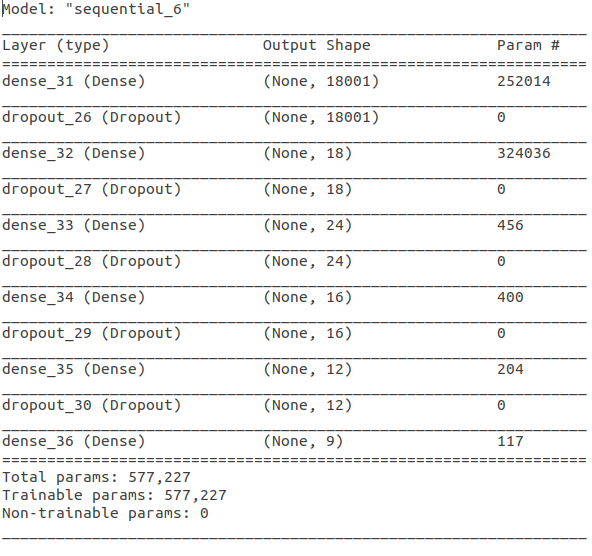
\includegraphics[scale=0.4]{./images/summary}
    \caption{Diagrama de funcionamiento offline}
    \label{fig:Red_offline}
\end{figure}

% \textbf{La red será implementada usando la biblioteca de redes neuronales \texttt{Keras}, la cual es biblioteca de Redes Neuronales OpenSource escrita en Python y está diseñada para facilitar la experimentación con redes de Deep Learning. Se caracteriza por ser amigable para el usuario, modular y extensible.}

% Un aspecto sumamente importante a mencionar es que si bien al finalizar el entrenamiento de la red, esta arroja un valor de precisión con que es capaz de predecir un valor de salida según valor de entrada dado, se tiene que este indicador no refleja con seguridad el comportamiento de la red. Es por esto, que nos valdremos de técnicas que arrojan ciertas otras métricas tales como varianza, precisión, exactitud y matriz de confusión, así como también, parámetros que permiten comprender con mayor certidumbre cómo se procesará y predecirá los datos nuestra red.

Es sobre estas capas en las que se aplicarán las técnicas de Cross-validation y Grid-Search para entregar información respecto de; cuál es el valor de las métricas que reflejan el comportamiento real de la red y cuáles son los parámetros (n$^\circ$ de capas y epochs, optimizador y batch-size) y con ello, optimizar el funcionamiento de la red. Cabe mencionar, que dentro de los indicadores que se obtendrán se encuentra la Matriz de Confusión, con esta se apoyará la exactitud y precisión de la red.
